\section{Графики задачи}
1. Построить график функции $y=\cfrac{|x+1|}{x+1}(x-1).$\\
2. Построить график функции $y=\cfrac{|x-1|}{x-1}(x+1).$\\
3. Построить график функции $f(x)=\cfrac{|x^2-4x+3|}{|x-1|}.$\\
4. Построить график функции $f(x)=\cfrac{|x^2-x-2|}{|x+1|}.$\\
5. Построить график функции $f(x)=\cfrac{|x^2-4x|}{x}+|-x|.$\\
6. Построить график функции $f(x)=\cfrac{|x^2-2x|}{x-2}+|x|.$\\
7. Построить график функции $f(x)=2x^2-8x+q,$ если сумма квадратов корней этой функции равна 10.\\
8. Построить график функции $f(x)=-2x^2+2x+q,$ если квадрат разности корней этой функции равен 9.\\
9. Найти центр симметрии графика функции $y=\cfrac{x+1}{x}.$\\
10. Найти центр симметрии графика функции $y=\cfrac{1-x}{x}.$\\
11. Найти расстояние от начала координат до прямой $3y+4x=12.$\\
12. Найти расстояние от начала координат до прямой $3y-4x=12.$\\
13. Найдите оси симметрии графика функции $y=|x+1|+|x+3|.$\\
14. Найдите оси симметрии графика функции $y=|x-1|+|x-3|.$\\
15. Для окружности, заданной уравнением $x^2+y^2-4x-6y=0$ найдите центр и радиус.\\
16. Для окружности, заданной уравнением $x^2+y^2+6x-4y+2=0$ найдите центр и радиус.\\
17. Постройте график функции $y=\cfrac{|x-2|}{2-x}(x^2-2x).$\\
18. Постройте график функции $y=\cfrac{|x+2|}{2+x}(x^2+4x+3).$\\
19. Построить график $y=\cfrac{x^2+7x+6}{x+|x+2|}.$\\
20. Построить график $y=\cfrac{x^2-6x+5}{x-|x-2|}.$\\
21. Дано изображение графика функции $y=ax^2+bx+c$ (см. рис.). Определить знаки коэффициентов $a,\ b,\ c.$ Не забудьте обосновать ответ.
$$\begin{tikzpicture}[scale=1]
\begin{axis}[
    axis lines = middle,
    legend pos={south west},
    %xlabel = {$x$},
    %xlabel style={below right},
    %ylabel = {$y$},
    %title={$\text{Рис. 2}$},
    ymin=-3,
    ymax=3.8,
    xmin=-3,
    xmax=3.5,
    xtick=\empty,
	ytick=\empty,
    ]
	\addplot[domain=-1.4:3.4, samples=100, color=black] {0.2*(x^2-2*x-3)};
	%\addlegendentry{$\text{Рис. 1}$};
\end{axis}
\draw (2.75,5.7) node {\scriptsize $y$};
\draw (7,2.2) node {\scriptsize $x$};
\end{tikzpicture}$$
22. Дано изображение графика функции $y=ax^2+bx+c$ (см. рис.). Определить знаки коэффициентов $a,\ b,\ c.$ Не забудьте обосновать ответ.
$$\begin{tikzpicture}[scale=1]
\begin{axis}[
    axis lines = middle,
    legend pos={south west},
    %xlabel = {$x$},
    %xlabel style={below right},
    %ylabel = {$y$},
    %title={$\text{Рис. 2}$},
    ymin=-3,
    ymax=3.8,
    xmin=-3,
    xmax=3.5,
    xtick=\empty,
	ytick=\empty,
    ]
	\addplot[domain=-1.4:3.4, samples=100, color=black] {-0.2*(x^2-2*x+7)};
	%\addlegendentry{$\text{Рис. 1}$};
\end{axis}
\draw (2.75,5.7) node {\scriptsize $y$};
\draw (7,2.2) node {\scriptsize $x$};
\end{tikzpicture}$$
23. Построить график функции $y=\cfrac{\sqrt{(x+1)^2-4x}}{x^2-x}.$\\
24. Построить график функции $y=\cfrac{\sqrt{(x-1)^2+4x}}{x^2+x}.$\\
25. Изобразить множество точек на плоскости: $(|y|-3)(y+|x|-1)=0.$\\
26. Изобразить множество точек на плоскости: $(|x|-3)(x+|y|-1)=0.$\\
27. Пусть $f(x)=\cfrac{x-2+|2x-1|}{x^2-1}.$\\
а) постройте график функции $y=f(x);$\\
б) найдите область определения и множество значений функции;\\
в) сколько решений имеет уравнение $f(x)=a$ в зависимости от $a?$\\
28. Пусть $f(x)=\cfrac{x+2-|2x+1|}{x^2-1}.$\\
а) постройте график функции $y=f(x);$\\
б) найдите область определения и множество значений функции;\\
в) сколько решений имеет уравнение $f(x)=a$ в зависимости от $a?$\\
29. Изобразите на координатной плоскости множество точек, координаты которых удовлетворяют уравнению $\cfrac{x^2+y^2-9}{x^2-y^2}=0.$\\
30. Изобразите на координатной плоскости множество точек, координаты которых удовлетворяют уравнению $\cfrac{x^2+y^2-1}{x^2-y^2}=0.$\\
31. Построить график $y=\cfrac{x-2}{|x^2-2x|}.$\\
32. Построить график $y=\cfrac{3-x}{|x^2-3x|}.$\\
33. Найти расстояние от начала координат до прямой $y=1-\cfrac{x}{2}.$\\
34. Найти расстояние от начала координат до прямой $y=2-2x.$\\
35. Задайте формулой квадратичную функцию, если её график проходит через точки $A(0;-2)$ и $B(-2;4)$ и функция принимает значение $-4$ в единственной точке.\\
36. Задайте формулой квадратичную функцию, если её значения при $x=-1$ и при $x=2$ совпадают, её наибольшее значение равно 3, а график содержит точку $P(1;1).$\\
37. Пусть $f(x)=\cfrac{x-1+|x-1|}{x^2-1}.$\\
а) постройте график функции $y=f(x);$\\
б) найдите область определения и множество значений функции;\\
в) сколько решений имеет уравнение $f(x)=a$ в зависимости от $a?$\\
38. Пусть $f(x)=\cfrac{x+1-|x+1|}{x^2-1}.$\\
а) постройте график функции $y=f(x);$\\
б) найдите область определения и множество значений функции;\\
в) сколько решений имеет уравнение $f(x)=a$ в зависимости от $a?$\\
39. Изобразите на координатной плоскости множество точек, координаты которых удовлетворяют уравнению $\cfrac{x^2-y^2}{x^2+y^2-9}=0.$\\
40. Изобразите на координатной плоскости множество точек, координаты которых удовлетворяют уравнению $\cfrac{x^2-y^2}{x^2+y^2-1}=0.$\\
41. Изобразите на координатной плоскости множество точек, координаты которых удовлетворяют уравнению $\cfrac{x^2-y^2}{x^2+y^2-4}=0.$\\
42. Изобразите на координатной плоскости множество точек, координаты которых удовлетворяют уравнению $\cfrac{x^2-y^2}{x^2+y^2-16}=0.$\\
43. Дана функция $f(x)=|x^2-2x|.$\\
а) постройте график функции $y=f(x);$\\
б) сколько решений имеет уравнение $f(x)=a$ в зависимости от $a?$\\
44. Дана функция $f(x)=|x^2+2x|.$\\
а) постройте график функции $y=f(x);$\\
б) сколько решений имеет уравнение $f(x)=a$ в зависимости от $a?$\\
45. Изобразите на координатной плоскости множество точек, координаты которых удовлетворяют уравнению $\cfrac{yx-x^2-y+1}{x-1}=0.$\\
46. Изобразите на координатной плоскости множество точек, координаты которых удовлетворяют уравнению $\cfrac{(y-2x+1)(y+2x-1)}{y^2-x^2}=0.$\\
47. Прямая $a$ проходит через точки с координатами $(0;4)$ и $(6;0).$ Прямая $b$ проходит через точку с координатами $(0;8)$ и параллельна прямой $a.$ Найдите абсциссу точки пересечения прямой $b$ с осью $Ox.$\\
48. Прямая $a$ проходит через точки с координатами $(-6;0)$ и $(0;4).$ Прямая $b$ проходит через точку с координатами $(0;-6)$ и параллельна прямой $a.$ Найдите абсциссу точки пересечения прямой $b$ с осью $Ox.$\\
49. $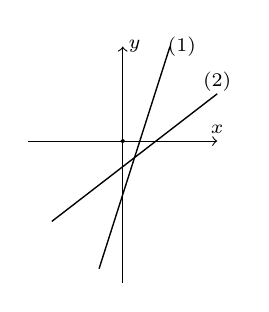
\begin{tikzpicture}[scale=0.6]
\tikzset {line01/.style={line width =0.5pt}}
\tikzset{line02/.style={line width =1pt}}
\tikzset{line03/.style={dashed,line width =0.9pt}}
\filldraw [black] (0,0) circle (1pt);
\draw [->] (-2,0) -- (2,0);
\draw [->] (0,-3) -- (0,2);
\draw[line01] (-1.5,-1.7) -- (2,1);
\draw[line01] (-0.5,-2.7) -- (1,2);
\draw (1.25,2) node {\scriptsize $(1)$};
\draw (2,1.25) node {\scriptsize $(2)$};
\draw (2,0.25) node {\scriptsize $x$};
\draw (0.25,2) node {\scriptsize $y$};
\end{tikzpicture}$ На рисунке изображены две прямые с уравнениями (1) $y_1=k_1x+b_1$ и (2)
$y_2=k_2x+b_2.$ Расставьте в порядке возрастания числа $k_1,\ k_2,\ b_1,\ b_2.$\\
50. $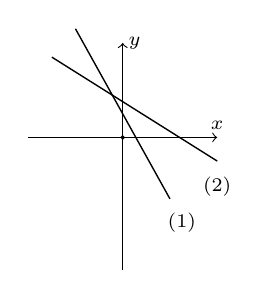
\begin{tikzpicture}[scale=0.6]
\tikzset {line01/.style={line width =0.5pt}}
\tikzset{line02/.style={line width =1pt}}
\tikzset{line03/.style={dashed,line width =0.9pt}}
\filldraw [black] (0,0) circle (1pt);
\draw [->] (-2,0) -- (2,0);
\draw [->] (0,-2.8) -- (0,2);
\draw[line01] (-1.5,1.7) -- (2,-0.5);
\draw[line01] (-1,2.3) -- (1,-1.3);
\draw (1.25,-1.8) node {\scriptsize $(1)$};
\draw (2,-1.05) node {\scriptsize $(2)$};
\draw (2,0.25) node {\scriptsize $x$};
\draw (0.25,2) node {\scriptsize $y$};
\end{tikzpicture}$ На рисунке изображены две прямые с уравнениями (1) $y_1=k_1x+b_1$ и (2)
$y_2=k_2x+b_2.$ Расставьте в порядке возрастания числа $k_1,\ k_2,\ b_1,\ b_2.$\\
51. а) Постройте график функции $y=-|x^2-2x|.$\\
б) При каких $a$ прямая $y=a$ пересекает график функции в двух точках?\\
52. а) Постройте график функции $y=|x^2-4x|.$\\
б) При каких $a$ прямая $y=a$ пересекает график функции в двух точках?\\
53. Парабола задана уравнением $y=(x+a)^2+1.$ Прямая, задаваемая уравнением $y=4+2x$ имеет с параболой единственную общую точку. Найти $a.$\\
54. Парабола задана уравнением $y=-(x-a)^2+4.$ Прямая, задаваемая уравнением $y=2x-5$ имеет с параболой единственную общую точку. Найти $a.$\\
55. Изобразите множество точек, координаты которых удовлетворяют условию $|xy|>1.$\\
56. Изобразите множество точек, координаты которых удовлетворяют условию $|xy|<1.$\\
57. а) Постройте график функции $y=-\cfrac{4(x+2)}{x^2+x-2}.$\\
б) Найдите число решений уравнения $y=a$ в зависимости от $a.$\\
58. а) Постройте график функции $y=\cfrac{2(x-1)}{3x-2-x^2}.$\\
б) Найдите число решений уравнения $y=a$ в зависимости от $a.$\\
59. Докажите, что прямая $2x+6y-9=0$ не проходит через точки, обе координаты которых --- целые числа.\\
60. Докажите, что прямая $4x+6y-7=0$ не проходит через точки, обе координаты которых --- целые числа.\\
61. Постройте график функции $f(x)=x^2-|2x-2|-1$ и укажите её множество значений.\\
62. Постройте график функции $f(x)=(x+1)|x-1|$ и укажите промежутки её возрастания.\\
63. Постройте график функции $y=\cfrac{(x^2+2x-8)(x+2)}{|x+2|}.$ При каких $m$ прямая $y=m$ пересекает график функции в трёх точках?\\
64. Постройте график функции $y=\cfrac{(x^2-4x+3)(x-1)}{|x-1|}.$ При каких $m$ прямая $y=m$ пересекает график функции в трёх точках?
ewpage

oindent65. Могут ли параболы на рисунке  быть графиками функций  $f(x)=ax^2+b_1x+c$ и $g(x)=cx^2+b_2x+a?$
$$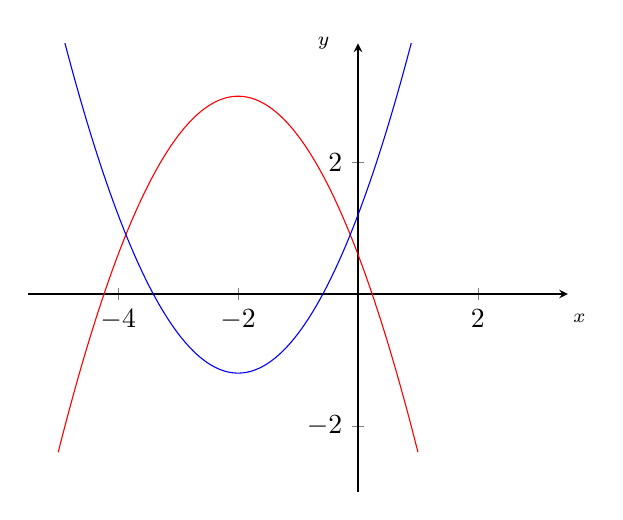
\begin{tikzpicture}[scale=1]
\begin{axis}[
    axis lines = middle,
    legend pos={south west},
    %xlabel = {$x$},
    %xlabel style={below right},
    %ylabel = {$y$},
    %title={$\text{Рис. 2}$},
    ymin=-3,
    ymax=3.8,
    xmin=-5.5,
    xmax=3.5,
    %xtick=\empty,
	%ytick=\empty,
    ]
	\addplot[domain=-5:1, samples=100, color=red] {-0.6*(x^2+4*x-1)};
	\addplot[domain=-5:1, samples=100, color=blue] {0.6*(x^2+4*x+2)};
%\addlegendentry{$\text{Рис. 1}$};
\end{axis}
\draw (3.75,5.7) node {\scriptsize $y$};
\draw (7,2.2) node {\scriptsize $x$};
\end{tikzpicture}$$
66. Могут ли параболы на рисунке  быть графиками функций  $f(x)=ax^2+b_1x+c$ и $g(x)=cx^2+b_2x+a?$
$$\begin{tikzpicture}[scale=1]
\begin{axis}[
    axis lines = middle,
    legend pos={south west},
    %xlabel = {$x$},
    %xlabel style={below right},
    %ylabel = {$y$},
    %title={$\text{Рис. 2}$},
    ymin=-5,
    ymax=3.8,
    xmin=-5.5,
    xmax=7.5,
    %xtick=\empty,
	%ytick=\empty,
    ]
	\addplot[domain=-3:7, samples=100, color=red] {-0.3*((x-4)^2+4*(x-4)-1)-2.5};
	\addplot[domain=-3:7, samples=100, color=blue] {0.3*((x-4)^2+4*(x-4)-5)};
%\addlegendentry{$\text{Рис. 1}$};
\end{axis}
\draw (2.75,5.7) node {\scriptsize $y$};
\draw (7,2.8) node {\scriptsize $x$};
\end{tikzpicture}$$
67. Постройте график функции $y=-\cfrac{4|x+2|}{x^2+2x}.$ При каком значении $m$ прямая $y=m$ имеет с графиком ровно одну общую точку?\\
68. Постройте график функции $y=-\cfrac{6|x-3|}{x^2-3x}.$ При каком значении $m$ прямая $y=m$ имеет с графиком ровно одну общую точку?\\
69. Постройте график функции $y=\cfrac{2x^2-8x}{|x-2|-2}$ и укажите те значения функции, которые она принимает ровно один раз.\\
70. Постройте график функции $y=\cfrac{3x^2-6x}{|x-1|-1}$ и укажите те значения функции, которые она принимает ровно один раз.\\
71. Может ли парабола, приведённая на рисунке (абсцисса её вершины равна 2), быть графиком функции $y=a(x-1)(x-4),$ где $a
eq0?$
$$\begin{tikzpicture}[scale=1]
\begin{axis}[
    axis lines = middle,
    legend pos={south west},
    %xlabel = {$x$},
    %xlabel style={below right},
    %ylabel = {$y$},
    %title={$\text{Рис. 2}$},
    ymin=-3,
    ymax=5.5,
    xmin=-1,
    xmax=6,
    %xtick=\empty,
	%ytick=\empty,
    ]
	\addplot[domain=-1:5, samples=100, color=black] {(2*x^2-8*x+5)};
	%\addplot[domain=-5:1, samples=100, color=blue] {0.6*(x^2+4*x+2)};
%\addlegendentry{$\text{Рис. 1}$};
\end{axis}
\draw (1.2,5.7) node {\scriptsize $y$};
\draw (7,2.2) node {\scriptsize $x$};
\end{tikzpicture}$$
72. Может ли парабола, приведённая на рисунке (абсцисса её вершины равна 3), быть графиком функции $y=a(x-2)(x-5),$ где $a
eq0?$
$$\begin{tikzpicture}[scale=1]
\begin{axis}[
    axis lines = middle,
    legend pos={south west},
    %xlabel = {$x$},
    %xlabel style={below right},
    %ylabel = {$y$},
    %title={$\text{Рис. 2}$},
    ymin=-3,
    ymax=5.5,
    xmin=-1,
    xmax=6,
    %xtick=\empty,
	%ytick=\empty,
    ]
	\addplot[domain=-1:6, samples=100, color=black] {(0.2*(3*x^2-18*x)+4)};
	%\addplot[domain=-5:1, samples=100, color=blue] {0.6*(x^2+4*x+2)};
%\addlegendentry{$\text{Рис. 1}$};
\end{axis}
\draw (1.2,5.7) node {\scriptsize $y$};
\draw (7,2.2) node {\scriptsize $x$};
\end{tikzpicture}$$
73. Постройте график функции $f(x)=-2x^{-2}$ при $x<0$ и $f(x)$ --- нечётная функция.\\
74. Постройте график функции $y=\cfrac{2x-3}{|x+2|}.$\\
75. Найдите все значения параметра $k,$ при которых гипербола $y=\cfrac{k}{x-2}$ пересекает прямую, задаваемую уравнением $y=x+1,$ в точке, лежащей на оси ординат.\\
76. Постройте график функции $y=\cfrac{x^3-x}{|x|}.$\\
77. Найдите все значения параметра $a,$ при которых прямая $y=a$ пересекает график функции $y=|x^2-4x|$ в двух точках.\\
78. Построить график функции $f(x)=\cfrac{|x^2-3x|(x+1)}{x}.$\\
79. Построить график функции $f(x)=\cfrac{|x^2+2x|(x-1)}{x}.$\\
80. Построить график функции $g(x)=\cfrac{2x+1}{2x^2+x}$ и определить:\\
а) при каких $k$ прямая $y=kx$ имеет одну общую точку с графиком функции $g(x)?$\\
б) при каких $b$ прямая $y=bx+2$ имеет одну общую точку с графиком функции $g(x)?$\\
81. Построить график функции $g(x)=\cfrac{x-2}{2x-x^2}$ и определить:\\
а) при каких $k$ прямая $y=kx$ имеет одну общую точку с графиком функции $g(x)?$\\
б) при каких $b$ прямая $y=bx+2$ имеет одну общую точку с графиком функции $g(x)?$\\
82. Пусть дана функция $f(x)=\cfrac{2-|x+3|}{x}.$\\
а) Постройте график функции $y=f(x),$\\
б) Решите неравенство $f(x)\geqslant-\cfrac{3}{2},$\\
в) Сколько корней имеет уравнение $f(x)=a$ в зависимости от $a?$\\
83. Пусть дана функция $f(x)=\cfrac{1-|x-2|}{x}.$\\
а) Постройте график функции $y=f(x),$\\
б) Решите неравенство $f(x)\leqslant\cfrac{3}{2},$\\
в) Сколько корней имеет уравнение $f(x)=a$ в зависимости от $a?$\\
84. Построить график функции $f(x)=\begin{cases} \sqrt{1-x},\ \text{ если } x\leqslant0,\\
x^2-|2x+1|,\ \text{ если } x>0.\end{cases}$\\
85. Пусть $f(x)=\begin{cases} 2, \text{ если } x>1,\\ -1, \text{ если } x<1,\\ 1, \text{ если } x=1.\end{cases}$\\
Постройте график $f(\sqrt{x-2}).$\\
86. Построить график функции $f(x)=\cfrac{1-|x-2|}{x}$ и решить неравенство $f(x)\leqslant 2.$\\
87. Построить график функции $f(x)=\cfrac{2-|x+3|}{x}$ и решить неравенство $f(x)\leqslant -2.$\\
88. Построить график функции $f(x)=|x^2-6x+5|$ и найти, при каком $k$ этот график имеет три общие точки с графиком функции $g(x)=k(x-7)+4.$\\
89. Построить график функции $f(x)=|x^2+2x-3|$ и найти, при каком $k$ этот график имеет три общие точки с графиком функции $g(x)=k(x+5)+4.$\\
90. а) Постройте график функции $f(x)=x^2-|2x-1|.$\\
б) При каких значениях параметра $a$ уравнение $x^2=|2x-1|+a$ имеет ровно два решения?\\
91. \begin{figure}[ht!]
\center{\includegraphics[scale=0.35]{grpar.png}}
\end{figure}\\
На рисунке параболы $f$ с уравнением $y=a_1 x^2+b_1x+c_1$ и $g$ с уравнением $y=a_2 x^2+b_2x+c_2$ касаются друг друга в точке, лежащей на оси ординат. Найдите соотношение между коэффициентами $a_1$ и $a_2;\ b_1$ и $b_2;\ c_1$ и $c_2.$\\
92. Постройте график функции $f(x)=\cfrac{x^2+x}{x}\cdot\sqrt{x^2-6x+9}.$\\
93. Постройте график функции $f(x)=\cfrac{x^2+x-6}{2-x}\cdot\sqrt{x^2-2x+1}.$\\
94. Известно, что графики функций $y=x^2+p$ и $y=-4x-5$ имеют ровно одну общую точку. Определите координаты этой точки. Постройте графики заданных функций в одной системе координат.\\
95. Изобразите на координатной плоскости множество точек, координаты которых удовлетворяют условию\\
(А) $|2x-y|=x;$\\
(Б) $|2x-y|<x.$\\
96. $f(x)=\begin{cases} \cfrac{3x-1}{x+1},\ x
eq-1\\a+2,\ x=-1 \end{cases}$\\
а) Построить график функции при $a=3.$\\
б) При каких $a$ уравнение $f(x)=a-1$ не имеет решений?\\
в) При каких $a$ прямая $y=ax+1$ имеет с графиком функции $f(x)$ три общие точки?\\
97. $f(x)=\begin{cases} \cfrac{3x+1}{x-1},\ x
eq1\\3-a,\ x=1 \end{cases}$\\
а) Построить график функции при $a=-1.$\\
б) При каких $a$ уравнение $f(x)=a+1$ не имеет решений?\\
в) При каких $a>0$ прямая $y=ax+2$ имеет с графиком функции $f(x)$ три общие точки?\\
98. $f(x)=\begin{cases} 4-|x+1|,\ x<2\\ x^2-6x+4,\ x\geqslant 2\end{cases}$\\
а) Построить график функции $f(x)$\\
б) При каких $a$ уравнение $f(x)=2a$ имеет два решения?\\
99. $f(x)=\begin{cases} |x-3|-4,\ x>1\\ -x^2-3x+4,\ x\leqslant 1\end{cases}$\\
а) Построить график функции $f(x)$\\
б) При каких $a$ уравнение $f(x)=\cfrac{a}{2}$ имеет два решения?\\
100. Постройте график функции $y=f(x),$ где $f(x)=\begin{cases}\cfrac{4}{x}, \text{ при } x<-2,\\
\cfrac{x}{2}-1, \text{ при } -2\leqslant x \leqslant 2,\\
x^2-6x+8, \text{ при } x>2.\end{cases}$\\
При каких значениях $m$ прямая $y = m$ имеет с графиком этой функции две общие точки?\\
101. Постройте график функции $y=f(x),$ где $f(x)=\begin{cases}-\cfrac{1}{x}, \text{ при } x\leqslant -1,\\
-x, \text{ при } -1< x \leqslant 1,\\
-x^2+4x-4, \text{ при } x>1.\end{cases}$\\
При каких значениях $m$ прямая $y = m$ имеет с графиком этой функции три общие точки?

ewpage
